% 第 17 题：半圆轨道 OPQS 与可绕 O 转动的金属杆 OM
% 原图：S 在左下、P 在右下、Q 为半圆弧中点（正上方），M 在弧上某处
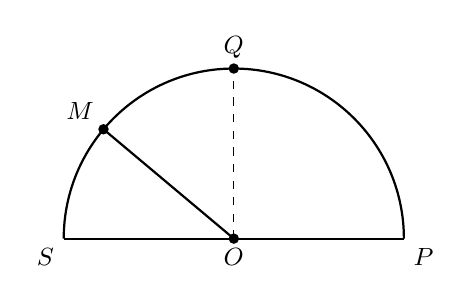
\begin{tikzpicture}[font=\small, scale=1.35]
  % 半圆弧（自 S 经 Q 到 P）
  \draw[thick] (180:1.6) arc[start angle=180, end angle=0, radius=1.6];
  % 直径 SP
  \draw[thick] (-1.6,0) -- (1.6,0);
  % 圆心 O
  \coordinate (O) at (0,0);
  \fill (O) circle (1.4pt) node[below] {$O$};
  % Q（弧中点）
  \fill (0,1.6) circle (1.4pt) node[above] {$Q$};
  \draw[dashed] (O) -- (0,1.6);
  % M（弧上一点，位于第二象限）
  \coordinate (M) at (140:1.6);
  \fill (M) circle (1.4pt) node[above left] {$M$};
  % 金属杆 OM
  \draw[thick] (O) -- (M);
  % S、P 标注
  \node[below left] at (-1.6,0) {$S$};
  \node[below right] at (1.6,0) {$P$};
\end{tikzpicture}
